\documentclass[8pt]{article}
\usepackage{fullpage,enumitem,amsmath,amssymb,graphicx}
\usepackage{graphicx} % This is a package for including graphics in your solution.
\usepackage{listings}
\usepackage{amsmath}
\usepackage{mathtools}
\usepackage[margin=0.5in]{geometry}

\DeclarePairedDelimiter{\ceil}{\lceil}{\rceil}

% Subsections will have partNumber.subsectionLetter headings
\renewcommand{\thesubsection}{\thesection.\alph{subsection}}
\newcommand{\norm}[1]{\lVert#1\rVert}

% Set nice font for included code
\lstset{basicstyle=\footnotesize\ttfamily,breaklines=true}
\setlength{\parindent}{0.25in}

\begin{document}

\section{Equations}

Optimal policy:
    $$ \pi^*(s) = argmax_{\pi} V^{\pi}(s) = argmax_{a \in A(s)} \sum_{s'} P(s' | s, a) V(s') $$
Bellman Equation:
    $$ V(s) = R(s) + \gamma \max_{a \in A(s)} \sum_{s'} P(s' | s, a) V(s') $$
Bellman Update:
    $$ V_{i+1}(s) \leftarrow B V_i = R(s) + \gamma \max_{a \in A(s)} \sum_{s'} P(s' | s, a) V_i(s') $$
Bellman=Contraction:
    $$ \norm{V} = \max_s \lvert V(s) \rvert $$
    $$ \norm{B V_i - B V_i'} \leq \gamma \norm{V_i - V_i'} $$
    $$ \norm{B V_i - V} \leq \gamma \norm{V_i - V} $$
Error of the estimate $V_i$:
    $$ \norm{V_i - V} $$
    % This is the bound on the initial state value error
    $$ \norm{V_0 - V} \leq 2 R_{max} / (1 - \gamma) $$
Bound on state values (utilities):
    $$ V(s) \leq \pm R_{max} / (1 - \gamma) $$
To get $\norm{V_i - V} \leq \epsilon$:
    $$ \gamma^N 2 R_{max} / (1 - \gamma) \leq \epsilon $$
    $$ N = \ceil[\Bigg]{\frac{log(2R_{max}/(\epsilon(1-\gamma)))}{log(1/\gamma)}} $$

If $\norm{V_{i+1} - V_i} \leq \epsilon (1 - \gamma) / \gamma$ then $\norm{V_{i+1} - V} < \epsilon$ \\

Policy loss is $\norm{V^{\pi_i} - V}$ and is connected to $V_i$:
\begin{center}
    if $\norm{V_i - V} < \epsilon$ then $\norm{V^{\pi_i} - V} < w\epsilon\gamma/(1-\gamma)$
\end{center}

\noindent Policy Iteration: \\
    \indent Policy Evaluation: Given a policy $\pi_i$, calculate $V_i = V^{\pi_i}$, the utility of each state if $\pi_i$ were t be executed. \\
    \indent Policy Improvement: Calculate a new MEU policy $\pi_{i+1}$, using one-step look-ahead based on $V_i$. \\
    \indent Terminate when policy improvement yields no change in the utilities. \\
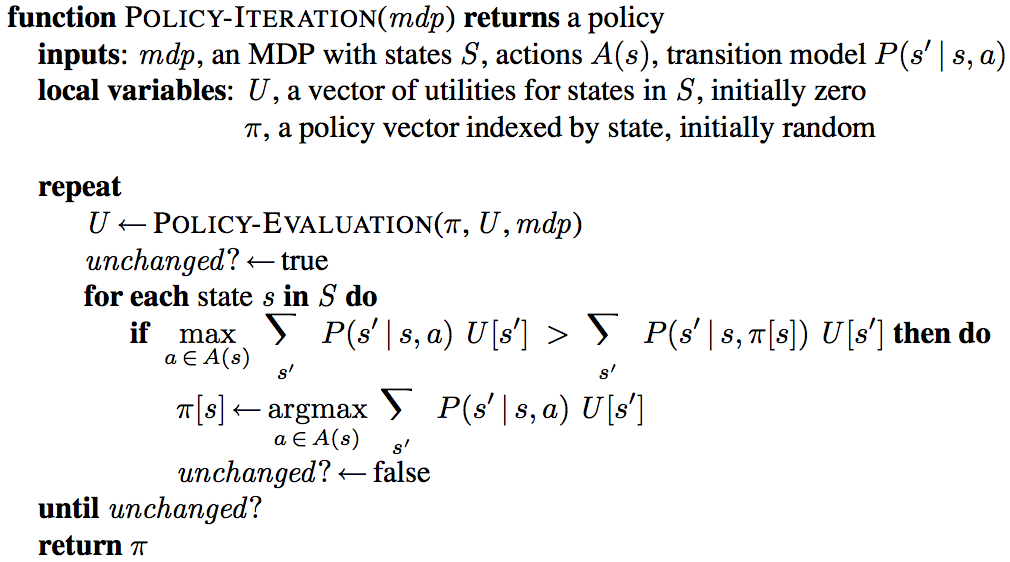
\includegraphics[width=10cm]{pics/policy_iteration.png}

\end{document}
